\section{Experimental Results}

% ========================================
% Experimental Setups Section
% ========================================
\subsection{Experimental Setups}
We carried out our experiments on DAS-4 using OpenNebula platform. The VM image we use is CentOS-5.4 whose image ID is 35, and our VM setup is CPU=1, VCPU=2, with 1024MB memory.

We prepared three H.264 1080p movie trailers downloaded from Apple Trailers\footnote{http://trailers.apple.com/trailers/}, which are described in Table \ref{table_joblist}:

\begin{table}[!t]
\caption{Jobs for Testings}
\label{table_joblist}
\centering
\begin{tabular}{|l|l|l|l|}
\hline
Job Name & File Name & Encoding & File Size\\
\hline
\texttt{job1} & cloudatlas-trailer1b\_h1080p.mov & H.264 1080p & 172MB \\
\hline
\texttt{job2} & skyfall-tlr2\_h1080p.mov & H.264 1080p & 180MB \\
\hline
\texttt{job3} & taken2-tlr1\_h1080p.mov & H.264 1080p & 175MB \\
\hline
\end{tabular}
\end{table}

For testing the provisioning policies, we created three different jobs with respect to these three files. Each job is to convert the H.264 1080p video file into an NTSC-DVD file. We then randomly generated three workloads, each of which comprises of 40 jobs. The job arrival times are generated using exponential distribution with three different parameters: 10, 20, and 30 seconds.

\begin{table}[!t]
\caption{Workloads for Testings}
\label{table_workloadlist}
\centering
\begin{tabular}{|l|l|l|}
\hline
Workload Name & Number of Jobs & Job Arrival Time Distribution \\
\hline
\texttt{wl-10} & 40 & Exponential(10) \\
\hline
\texttt{wl-20} & 40 & Exponential(20) \\
\hline
\texttt{wl-30} & 40 & Exponential(30) \\
\hline
\end{tabular}
\end{table}


% ========================================
% Experiments
% ========================================
\subsection{Experiments}

% ========================================
% Benchmark Tests
% ========================================
\subsubsection{Benchmark Tests}
First, we did some benchmark tests to measure the performance of DAS-4 OpenNebula. The benchmark consists of four tests:

\begin{enumerate}
\item The first three tests are using ffmpeg to convert the three video files separately. Each test was done by 20 times, and we measure the job's running times (the total amount of time a job spent on its execution).
\item Another test is continuously allocating and releasing a VM instance, in order to measure the overhead of allocating a VM instance on DAS-4.
\end{enumerate}

\begin{figure}[!t]
\centering
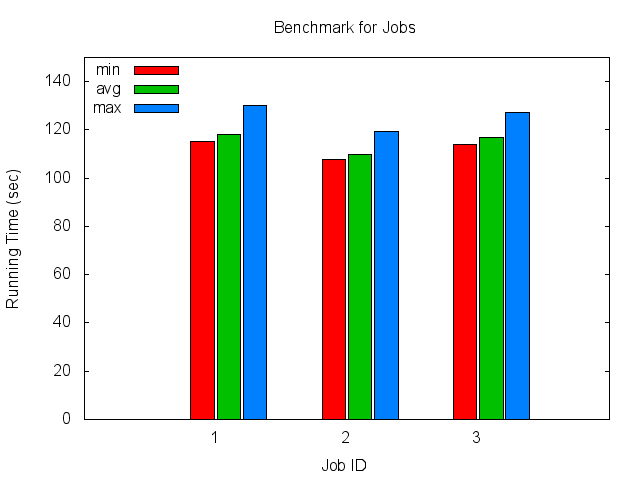
\includegraphics[width=0.35\textwidth]{pictures/bench-jobs.png}
\caption{Results of the benchmark tests for jobs}
\label{figure_jobbenchmark}
\end{figure}

As illustrated in Figure \ref{figure_jobbenchmark}, it is obvious that the performances of all jobs are almost the same, with an average of 114.819 seconds. The maximum and minimum values are also close to the averages.

For the VM allocation overhead test, we continuous allocate and release a VM instance for 20 times, and we measure its total preparation time, which is from the time it is allocated until the time it is accessible through SSH. The results are shown in Table \ref{table_vm_preparation}.

\begin{table}
\caption{Total Preparation Time of VMs}
\label{table_vm_preparation}
\centering
\begin{tabular}{|l|l|}
\hline
Average Total Preparation Time & 60.309 seconds \\
\hline
Average Allocation Time & $\approx$10 seconds \\
\hline
Average OS Booting Time & $\approx$50 seconds \\
\hline
\end{tabular}
\end{table}

We only show the average values because the minimum and maximum values are close to it. The allocation time is from the VM instance is allocated until its state becomes RUNNING, and the OS booting time is the time after that and until this VM is accessible through SSH.

The results suggest that the DAS-4 OpenNebula is efficient in allocating a VM instance. It only takes approximately 10 seconds to become RUNNING after it is allocated. However, it still needs 50 seconds to be able to use.


% ========================================
% Experiments on the Provisioning Policies
% ========================================
\subsection{Experiments on the Provisioning Policies}
In this part, we use the three workloads to test the two policies. We will just call STATIC for static policy, and SE for simple elastic policy for short, and SE with threshold set to 0 will be denoted as SE-0. Figure \ref{figure_jobmakespan} illustrates the job makespans using different policies in each workload.

\begin{figure}[!t]
\centering
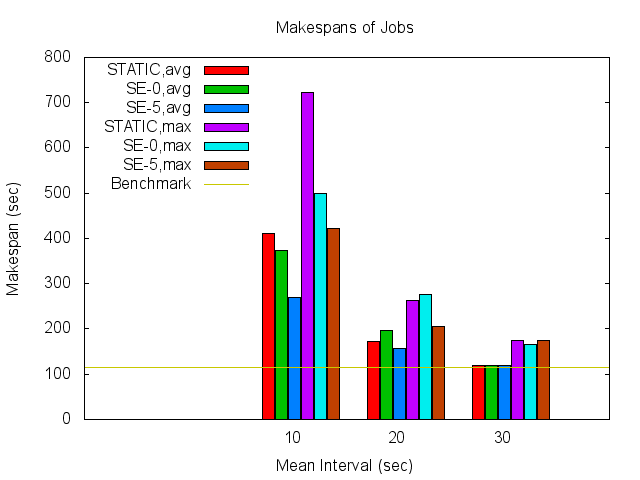
\includegraphics[width=0.35\textwidth]{pictures/all-makespans.png}
\caption{Makespans of jobs in the three workloads}
\label{figure_jobmakespan}
\end{figure}

The brown line there is the benchmark line indicating the average running time of a job. As expected, for \texttt{wl-10}, SE out performs the STATIC both in average case and worst case, and SE-5 has a much better performance than SE-0. For \texttt{wl-30}, the performances are almost the same. This suggests that five VMs are enough for \texttt{wl-30}.

What is worth noticing is that in \texttt{wl-20}, STATIC has the best performance. One explanation is that, our SE policy terminates an idle VM instance once the pending job queue becomes empty. In \texttt{wl-20}, the arriving of jobs is neither frequent, nor slow. So the pending job queue could get empty for several times. This scenario becomes a bottleneck of our SE policy, especially SE-5, because it only allocates more VMs when the number of pending jobs gets higher than 5.

\begin{figure}[!t]
\centering
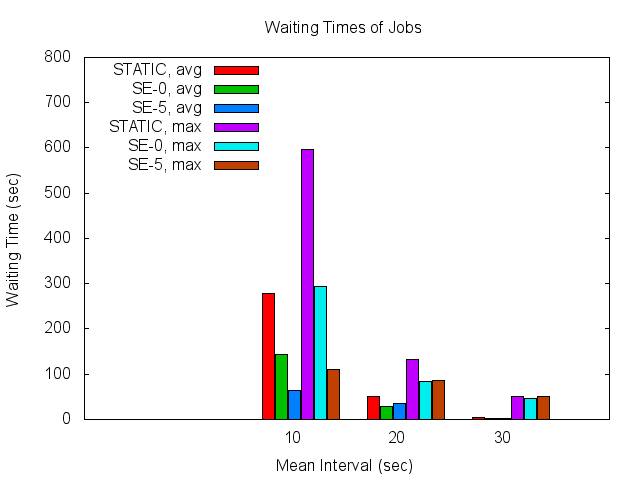
\includegraphics[width=0.35\textwidth]{pictures/all-waittimes.png}
\caption{Waiting times of jobs in the three workloads}
\label{figure_jobwaittime}
\end{figure}

Figure \ref{figure_jobwaittime} shows the waiting times of jobs. In \texttt{wl-20}, ES-0 has a lower waiting time than STATIC, however the overall makespan is higher. The makespan may be dragged down by the uploading and download overheads.

\begin{figure}[!t]
\centering
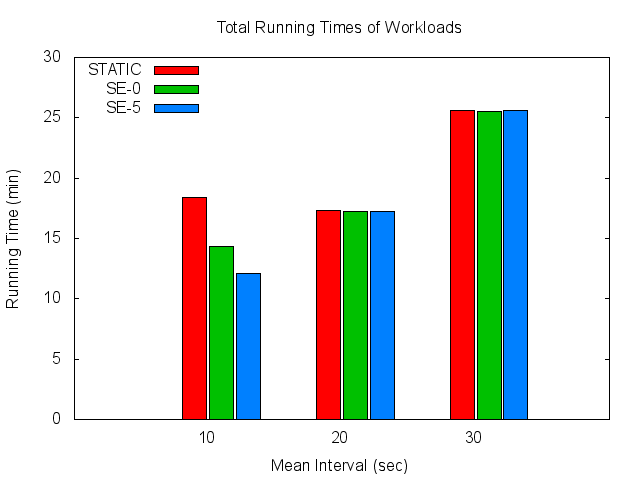
\includegraphics[width=0.35\textwidth]{pictures/workload-runtime.png}
\caption{Total makespan of three workloads}
\label{figure_workloadmakespan}
\end{figure}

Looking at the total makespans of each workload in Figure \ref{figure_workloadmakespan}, we observe that in \texttt{wl-10} and \texttt{wl-20}, SE works better than STATIC.


% ========================================
% VM Performance Section
% ========================================
\subsection{VM Performances}
We analyze the utilization of VMs in our system in this part. The utilization level is the fraction of time VMs spent on running jobs with respect to their total lifetime, and it can be described by Equation \ref{equation_vm_util}.

\begin{equation}
\label{equation_vm_util}
Utilization = \frac{\sum{T_{running\_jobs}}}{\sum{T_{lifetime}}}
\end{equation}

\begin{figure}[!t]
\centering
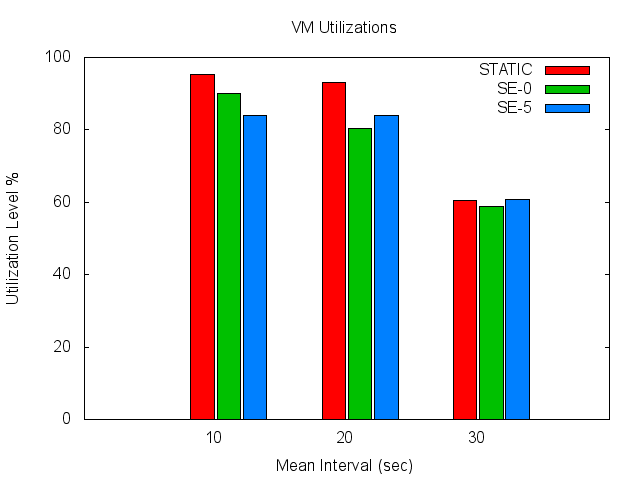
\includegraphics[width=0.35\textwidth]{pictures/vm-util.png}
\caption{VM Utilizations Levels}
\label{figure_vm_util}
\end{figure}

The results are depicted in Figure \ref{figure_vm_util}. Although in \texttt{wl-10} and \texttt{wl-20}, the utilization levels of SE are lower than STATIC, the decrements are acceptable. This suggests that SE can utilize the VMs relatively efficiently.

Due to SE's feature that it terminates an idle VM as soon as there is no pending jobs, we would also like to analyze its drawback and overhead. For doing this, we measure the number of wasted VMs by using SE. A VM can be wasted in this scenario: suppose we are using SE-0, and there are 5 VMs in the system with 5 jobs running on them respectively. Then a new job comes, and SE-0 will allocate a new VM, say $VM_{new}$. However, before $VM_{new}$ becomes available, one running job has been finished, which means a VM becomes idle, and this new job is then assigned to this free VM. So, when $VM_{new}$ is ready, the pending job queue is empty, and according to our policy, $VM_{new}$ is terminated. In this case, no job has been running on $VM_{new}$ during its lifetime, and we say that $VM_{new}$ is wasted.

In Figure \ref{figure_vm_wasted}, we can see that in \texttt{wl-10}, SE-5 gets a surprisingly low number of wasted VMs, while the number of SE-0 is as high as 60\%.

\begin{figure}[!t]
\centering
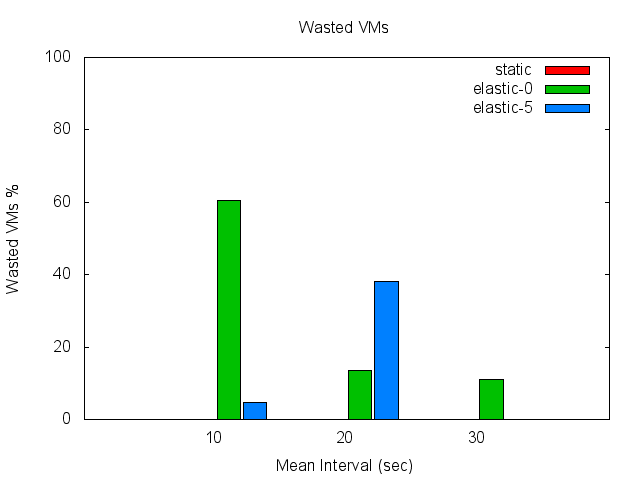
\includegraphics[width=0.35\textwidth]{pictures/vm-wasted.png}
\caption{Wasted VMs}
\label{figure_vm_wasted}
\end{figure}


% ========================================
% Speedup vs. Cost Tradeoff Section
% ========================================
\subsection{Speedup vs. Cost Tradeoff}
In this part, we calculate the speedups of using our SE provisioning policy and the charged-costs. Because our VM setup has no corresponding machine on Amazon Web Service, we use the charged cost of m1.medium (\$0.16 per hour for Linux), which has two compute units, for our charged-cost calculation. Table \ref{table_chargedcosts} shows the results.

\begin{table}
\caption{Charged-costs}
\label{table_chargedcosts}
\centering
\begin{tabular}{|l|l|l|l|}
\hline
Workload & STATIC & SE-0 & SE-5 \\
\hline
\texttt{wl-10} & 1.54hrs (\$0.246) & 2.86hrs (\$0.458) & 2.73hrs (\$0.437) \\
\hline
\texttt{wl-20} & 1.44hrs (\$0.230) & 2.32hrs (\$0.371) & 2.13hrs (\$0.341) \\
\hline
\texttt{wl-30} & 2.13hrs (\$0.341) & 2.18hrs (\$0.349) & 2.13hrs (\$0.341) \\
\hline
\end{tabular}
\end{table}

\begin{table}
\caption{Speedups and Costs for wl-10}
\label{table_speedupcost}
\centering
\begin{tabular}{|l|l|l|}
\hline
 & SE-0 & SE-5 \\
\hline
Speedup & 1.28 & 1.52 \\
\hline
Cost & 1.86 & 1.78 \\
\hline
\end{tabular}
\end{table}

We mainly focus on the results of \texttt{wl-10}, because this is the only case that SE outperforms STATIC. From Table \ref{table_speedupcost}, we can see that only SE-5 is close to cost-speed proportional in \texttt{wl-10}. The results suggest that the cost is usually higher than the performance you can gain. It is not an easy task to achieve a cost-efficient cloud application.
